
\newcommand{\IncludePerfProfSubFiguresBatchOne}[1]{
	\begin{subfigure}{0.30\textwidth}
		\centering
		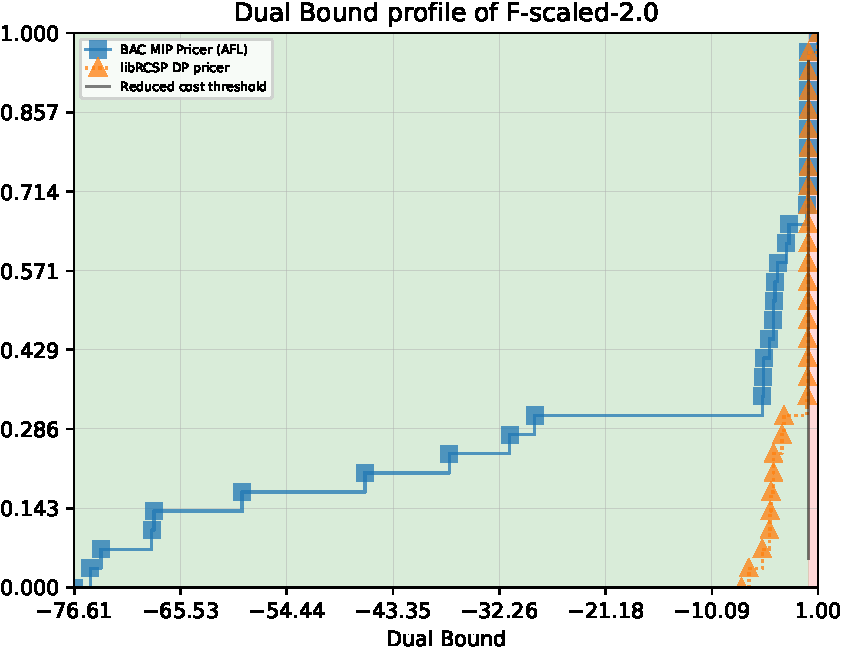
\includegraphics[width=1.0\linewidth]{./Imgs/perfprofs/#1/DualBound_plot.cropped.pdf}
	\end{subfigure}
}

\begin{figure}[t]
	\IncludePerfProfSubFiguresBatchOne{Fractional-labeling-comparison-for-E-scaled-1.0}
	\hfill
	\IncludePerfProfSubFiguresBatchOne{Fractional-labeling-comparison-for-E-scaled-2.0}
	\hfill
	\IncludePerfProfSubFiguresBatchOne{Fractional-labeling-comparison-for-E-scaled-4.0}

	\IncludePerfProfSubFiguresBatchOne{Fractional-labeling-comparison-for-F-scaled-1.0}
	\hfill
	\IncludePerfProfSubFiguresBatchOne{Fractional-labeling-comparison-for-F-scaled-2.0}
	\hfill
	\IncludePerfProfSubFiguresBatchOne{Fractional-labeling-comparison-for-F-scaled-4.0}

	\IncludePerfProfSubFiguresBatchOne{Fractional-labeling-comparison-for-A-scaled-1.0}
	\hfill
	\IncludePerfProfSubFiguresBatchOne{Fractional-labeling-comparison-for-A-scaled-2.0}
	\hfill
	\IncludePerfProfSubFiguresBatchOne{Fractional-labeling-comparison-for-A-scaled-4.0}

	\IncludePerfProfSubFiguresBatchOne{Fractional-labeling-comparison-for-B-scaled-1.0}
	\hfill
	\IncludePerfProfSubFiguresBatchOne{Fractional-labeling-comparison-for-B-scaled-2.0}
	\hfill
	\IncludePerfProfSubFiguresBatchOne{Fractional-labeling-comparison-for-B-scaled-4.0}

	\IncludePerfProfSubFiguresBatchOne{Fractional-labeling-comparison-for-P-scaled-1.0}
	\hfill
	\IncludePerfProfSubFiguresBatchOne{Fractional-labeling-comparison-for-P-scaled-2.0}
	\hfill
	\IncludePerfProfSubFiguresBatchOne{Fractional-labeling-comparison-for-P-scaled-2.0}

	\caption{
		This empirical study investigates the tightness of the dual bound for various versions of the BAC algorithm.
		The plots are laid out in a matrix format.
		Each row corresponds to a unique CVRP test set.
		From top to bottom: \texttt{E}, \texttt{F}, \texttt{A}, \texttt{B} and finally \texttt{P}.
		Each column represents a different inflation scale factor $s$.
		From left to right: $s = 1$, $s = 2$ and finally $s = 4$.
		The version that uses amortized fractional labeling (\texttt{AFL}), represented here by the orange line, appears to produce tighter dual bounds in the majority of cases.
	}
	\label{fig:perfprofs-batch1-part1}
\end{figure}
